\documentclass{beamer}
\usepackage{mathtools}
\usepackage{amsmath}
\usetheme{CambridgeUS}

\title{Receive Antenna Selection in MIMO Systems}
\author{Sandeep H M \and Dinesh Kumar Sonkar}
\date{\today}
\subject{EE5327 - Optimization}

\begin{document}

\begin{frame}
  \titlepage
\end{frame}

\section{Objective of the Paper}
\begin{frame}{Objective of the Paper}
\begin{itemize}
    \item The paper aims to maximize the channel capacity of the MIMO system.
    \vskip 0.2 in
    \item Reduce the cost of the system
    \vskip 0.2 in
    \item Optimization problem is solved using low complexity techniques
\end{itemize}
\end{frame}

\section{Convex Optimization Problem}
\begin{frame}{Convex Optimization Problem}
Maximize 
\begin{align*}
\mathnormal{C}_r(\mathbf{\Delta}) &=\log_{2}\text{det}(\mathbf{I}_M + \gamma\mathbf{\Delta}\textbf{H}\textbf{H}^H)
\end{align*}
subject to
$$0\leq\Delta_{i}\leq1,\enspace i=1,2,...,M$$
$$trace(\mathbf{\Delta})=\sum_{i=1}^{M} \Delta_i = M'$$
where
\vskip 0.1 in
$\mathnormal{C}_r(\mathbf{\Delta})$ is channel capacity\\
\textbf{H} is the M$\times$N channel matrix.
\end{frame}

\section{Proof}
\begin{frame}{Proof of Concavity}

We define g(t) = $\log|\mathbf{X}+t\mathbf{V}|$ such that $\mathbf{X}\in\mathnormal{S}_{++}^N$ and $\mathbf{V}\in\mathnormal{S}^N$
\begin{align*}
g(t) &= \log |\mathbf{X}+t\mathbf{V}|\\
&= \log|\mathbf{X}|+\sum_{i=1}^{N}\log(1+t\mathnormal{\lambda}_i)\\
\end{align*}
$$g''(t) = \sum_{i=1}^{N}\frac{-\mathnormal{\lambda}_i^2}{(1+t\mathnormal{\lambda}_i)^2}$$
Since $\mathrm{g}''(t)< 0 \mathrm{g}$(t) is concave\\
\vskip 0.1 in
$\Rightarrow \log|\mathbf{X}|$ is concave 
\end{frame}

\begin{frame}{Result}
\begin{figure}[h]
\centering
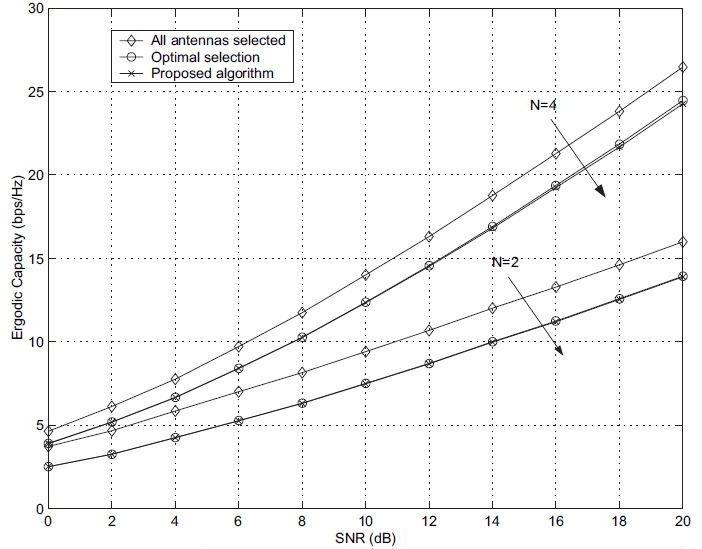
\includegraphics[width=0.6\textwidth]{SNR.JPG}
\caption{Ergodic capacity v/s SNR (N$_\gamma$), M = 6, N = 2,4 M' = N}
\end{figure}
\end{frame}

\section{System Model}
\begin{frame}{System Model}
Received signal can be represented as 
\begin{equation*}
    x(k) =\sqrt{E_s}\boldsymbol{H}s(k)+ \boldsymbol{n}(k)
\end{equation*}
where\\
\vskip 0.1in
x(k) is the $k^{th}$ sample of the received signal.\\
\vskip 0.1in
s(k) is the $k^{th}$ sample of the transmitted signal.\\
\vskip 0.1in
$E_s$ is the average energy per receive antenna and per channel use\\
\vskip 0.1in
n(k)  is AWGN with energy $\textstyle\frac{N_0}{2}$\\
\vskip 0.1in
\textbf{H} is the M$\times$N channel matrix.
\end{frame}
\section{Receive Antenna Selection In MIMO Systems}
\begin{frame}{Receive Antenna Selection In MIMO Systems}
`\textbf{Objective} - Select receive antenna to maximize capacity.\\
The capacity of a system is given by the formula
\begin{equation*}
    C(\boldsymbol{H})=\log_{2}\text{det}(\boldsymbol{I}_{N} + \gamma\boldsymbol{R}_{ss}\boldsymbol{H}^{H}\boldsymbol{H})
\end{equation*}
where\\
\vskip 0.2in
\gamma = \textstyle\frac{E_s}{N_0}
\newline
\newline
\mathbf{R}$_{ss}$ = E[s(k)s(k)$^H$] is the co-variance matrix of the transmitted signals with trace(\textbf{R}$_{ss}$)=1
\end{frame}

\begin{frame}{}
When only M'$<$M receive antennas are used, the capacity becomes a function of the antennas chosen.\\
\vskip 0.2in
We represent the indices of the selected antennas by r =
[r$_1$, . . . , r$_{M'}$]\\
\vskip 0.2in
The effective channel matrix becomes \textbf{H}$_r$ which is a M'$\times$N matrix.\\
\vskip 0.2in
The channel capacity with antenna selection is given by
\begin{equation*}
    C_r(\boldsymbol{H}_r) = \log_{2}\text{det}(\boldsymbol{I}_{N} + \gamma\boldsymbol{R}_{ss}\boldsymbol{H}_{r}^{H}\boldsymbol{H}_{r})
\end{equation*}
\end{frame}

\section{ANTENNA SELECTION AS AN OPTIMIZATION PROBLEM}
\begin{frame}{Antenna Selection as an Optimization Problem}`
We define \Delta$_i$
\[ \Delta_i = 
     \begin{cases}
       \text{1,} & \quad\text{if}\quad i$^{th}$ antenna is selected\\
       \text{0,} &\quad\text{otherwise.} \\ 
     \end{cases}
\]

Now, consider an M$\times$M diagonal matrix $\mathbf{\Delta}$ that has $\Delta_i$ as its diagonal entries.\\
Let us denote F =  $\mathbf{\Delta}$H.\\
F can be written as \textbf{H}$_r$ with (M-M') zero rows appended
to it and left multiplied by a M ×M row-permutation matrix P. Thus,
\begin{equation*}
    \boldsymbol{F} = \boldsymbol{P}
     \begin{bmatrix}
    \boldsymbol{H}_r\\
    0 _{(M-M')\times N}
\end{bmatrix}
= \boldsymbol{P}\widetilde{\boldsymbol{H}_{r}}
\end{equation*}
\end{frame}

\begin{frame}{}
Since P is a permutation matrix, \textbf{P$^H$}\textbf{P} = \textbf{I}$_M$.
\begin{align*}
\textbf{F}^H\textbf{F} &= \widetilde{\boldsymbol{H}_{r}}^H\textbf{P}^H\textbf{P}\widetilde{\boldsymbol{H}_{r}}\\
&= \widetilde{\boldsymbol{H}_{r}}^H\widetilde{\boldsymbol{H}_{r}}\\
&= \textbf{H}_r^H\textbf{H}_r
\end{align*} 
The channel capacity as a function of $\mathbf{\Delta}$ is
\begin{align*}
\mathnormal{C}_r(\mathbf{\Delta}) &=\log_{2}\text{det}(\mathbf{I}_N + \gamma\textbf{F}^H\textbf{F})\\
&= \log_{2}\text{det}(\mathbf{I}_N + \gamma\textbf{H}^H\mathbf{\Delta}^H\mathbf{\Delta}\textbf{H})
\end{align*}
\end{frame}

\begin{frame}{}
Since $\mathbf{\Delta}$ is a diagonal matrix with entries either 0 or 1\\
$$\mathbf{\Delta}^H\mathbf{\Delta}=\mathbf{\Delta}$$
The MIMO channel capacity with antenna selection can be re-written as
\begin{align*}
\mathnormal{C}_r(\mathbf{\Delta}) &=\log_{2}\text{det}(\mathbf{I}_N + \gamma\textbf{H}^H\mathbf{\Delta}\textbf{H})
\end{align*}
Using the identity det(\textbf{I$_m$} + \textbf{A}\textbf{B}) = det(\textbf{I}$_n$ + \textbf{B}\textbf{A}) we get
\begin{align*}
\mathnormal{C}_r(\mathbf{\Delta}) &=\log_{2}\text{det}(\mathbf{I}_M + \gamma\mathbf{\Delta}\textbf{H}\textbf{H}^H)
\end{align*}
\end{frame}

\begin{frame}{}
Maximize 
\begin{align*}
\mathnormal{C}_r(\mathbf{\Delta}) &=\log_{2}\text{det}(\mathbf{I}_M + \gamma\mathbf{\Delta}\textbf{H}\textbf{H}^H)
\end{align*}
subject to
$$0\leq\Delta_{i}\leq1,\enspace i=1,2,...,M$$
$$trace(\mathbf{\Delta})=\sum_{i=1}^{M} \Delta_i = M'$$
\end{frame}

\begin{frame}{Proof of Concavity}

We define g(t) = $\log|\mathbf{X}+t\mathbf{V}|$ such that $\mathbf{X}\in\mathnormal{S}_{++}^N$ and $\mathbf{V}\in\mathnormal{S}^N$
\begin{align*}
g(t) &= \log |\mathbf{X}+t\mathbf{V}|\\
&= \log|\mathbf{X}^{\frac{1}{2}}\mathbf{X}^{\frac{1}{2}}+t\mathbf{X}^{\frac{1}{2}}\mathbf{X}^{\frac{-1}{2}}\mathbf{V}\mathbf{X}^{\frac{-1}{2}}\mathbf{X}^{\frac{1}{2}}|\\
&= \log|\mathbf{X}^{\frac{1}{2}}(\mathbf{I} + t\mathbf{X}^{\frac{-1}{2}}\mathbf{V}\mathbf{X}^{\frac{-1}{2}})\mathbf{X}^{\frac{1}{2}}|\\
&= \log|\mathbf{X}^{\frac{1}{2}}(\mathbf{I} + t\mathbf{U}\mathbf{\Lambda}\mathbf{U}^{T})\mathbf{X}^{\frac{1}{2}}|\\
&= \log|\mathbf{X}^{\frac{1}{2}}\mathbf{U}(\mathbf{I} + t\mathbf{\Lambda})\mathbf{U}^{T}\mathbf{X}^{\frac{1}{2}}|\\
&= \log|\mathbf{X}^{\frac{1}{2}}||\mathbf{U}||\mathbf{I} + t\mathbf{\Lambda}||\mathbf{U}^{T}||\mathbf{X}^{\frac{1}{2}}|\\
&= \log|\mathbf{X}||\mathbf{I}+t\mathbf{\Lambda}|\\
&= \log|\mathbf{X}|+\log|\mathbf{I}+t\mathbf{\Lambda}|
\end{align*}
\end{frame}

\begin{frame}{}
\begin{align*}
    g(t) &= \log|\mathbf{X}|+\log|\mathbf{I}+t\mathbf{\Lambda}|\\
&= \log|\mathbf{X}|+\log(\prod_{i=1}^{N}1+t\mathnormal{\lambda}_i)\\
&= \log|\mathbf{X}|+\sum_{i=1}^{N}\log(1+t\mathnormal{\lambda}_i)
\end{align*}
$$g''(t) = \sum_{i=1}^{N}\frac{-\mathnormal{\lambda}_i^2}{(1+t\mathnormal{\lambda}_i)^2}$$
Since $\mathrm{g}''(t)< 0 \mathrm{g}$(t) is concave\\
\vskip 0.1 in
$\Rightarrow \log|\mathbf{X}|$ is concave     
\end{frame}

\section{Result}

\begin{frame}{Result}
Receive antenna selection has been approximated to a convex relaxation  that can be solved using low complexity techniques. It is of order O(M$^{3.5}$)\\
\vskip 0.1in
The selection algorithm gives an Ergodic capacity which is very close to the optimal one
\begin{figure}[h]
\centering
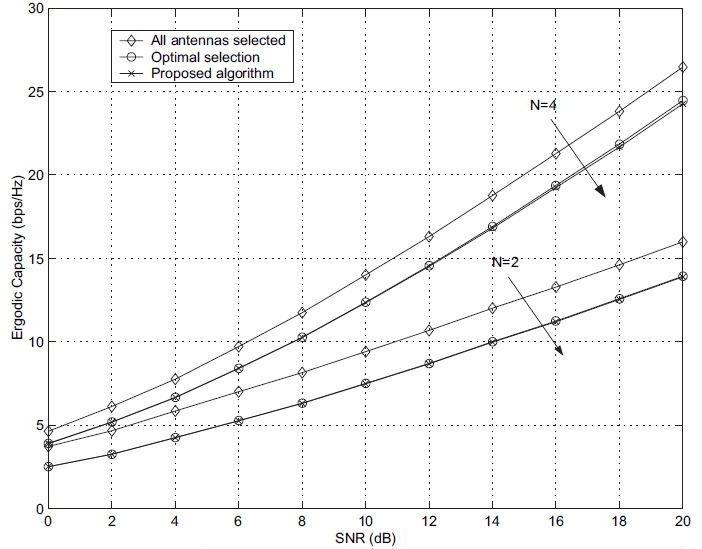
\includegraphics[width=0.3\textwidth]{SNR.JPG}
\caption{Ergodic capacity v/s SNR (N$_\gamma$), M = 6, N = 2,4 M' = N}
\end{figure}
\end{frame}

\end{document}